\section{Bayesian Analysis}


\subsection{Analysis of Normal Mean}

\begin{frame}{Bayesian Analysis of Normal Mean}

  \begin{itemize}
    \item Data $X | \mu \sim N(\mu, \sigma^2)$
    \item Conjugate prior $\mu \sim N(u, v)$
    \item Theoretically, posterior is $\mu | \bar{x} \sim N(u', v')$ where:
    \[ u' = \left(u \sigma^2 + v \sum_{i = 1}^{n} x_i\right) / (n v + \sigma^2) \]
    \[ v' = v \sigma^2/(n v + \sigma^2) \]
    \item We can see that the posterior mean is a linear combination of the prior mean and likelihood mean:
    \[ u' = w_n \cdot u + (1 - w_n) \cdot \sum_{i = 1}^{n} x_i / n \]
    where $w_n = \frac{\sigma^2 / n}{v + \sigma^2 / n}$
  \end{itemize}
  
\end{frame}

\begin{frame}{Bayesian Analysis of Normal Mean}

  \begin{itemize}
    \item We can see that $\lim_{n \to \infty} w_n = 0$
    \item As the data size increases, the posterior mean shifts towards the likelihood mean
    \item Also, $\frac{1}{v'} = \frac{1}{v} + \frac{n}{v^2}$, where $\frac{1}{v'}$ is the posterior precision
  \end{itemize}

  \begin{figure}
    \centering
    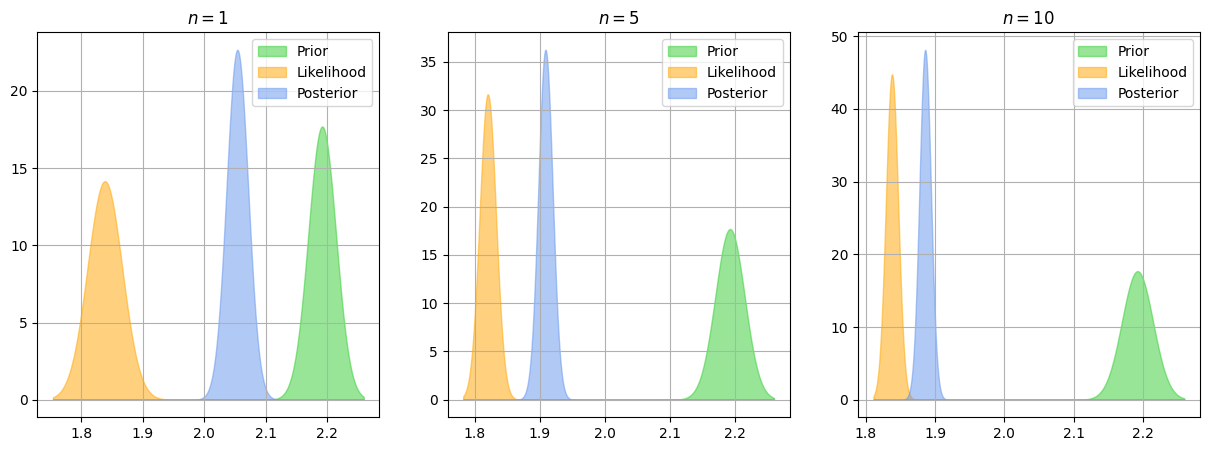
\includegraphics[width=\textwidth]{../Report/images/posterior.png}
    \caption{Posterior Analysis}
  \end{figure}

\end{frame}


\subsection{Central Posterior Interval}

\begin{frame}{Central Posterior Interval}

  \begin{itemize}
    \item Central Posterior Interval or credible interval of confidence level $\alpha$ is $[a, b]$ such that:
    \[ P(\mu | \bar{x} \in [a, b]) = \alpha \]
    \item Credible intervals are not unique
    \item High Density Interval (HDI) is the smallest credible interval.
  \end{itemize}

  \begin{figure}
    \centering
    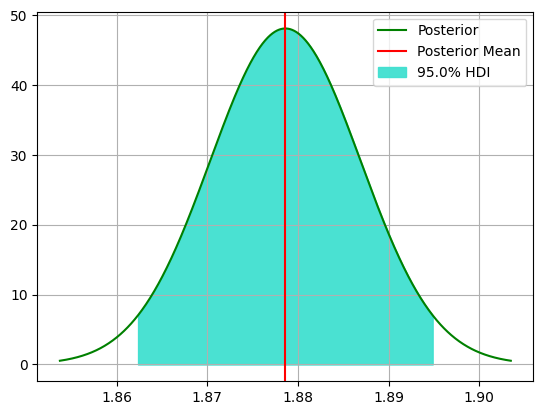
\includegraphics[width=.6\textwidth]{../Report/images/hdi.png}
    \caption{95\% posterior HDI}
  \end{figure}
  
\end{frame}
